% ROZDZIAŁ 2: Budowa stanowiska i oprogramowanie

\chapter{Budowa stanowiska i oprogramowanie}
\label{ch:budowa}

Niniejszy rozdział opisuje fizyczną budowę stanowiska laboratoryjnego, zastosowane
komponenty elektroniczne, środowisko programistyczne oraz architekturę oprogramowania
sterującego — firmware mikrokontrolera i~aplikację nadzorczą.

% -----------------------------------------------------------------------
\section{Opis stanowiska laboratoryjnego}
% -----------------------------------------------------------------------

Stanowisko składa się z~wydrukowanej w~technologii 3D pochyłej belki, po której
swobodnie toczy się kulka (pileczka ping pongowa).
Kąt nachylenia belki kontrolowany jest przez serwomechanek połączony z~belką
za pomocą dźwigni.
Pozycja kulki mierzona jest bezdotykowo za pomocą zaimplementowanego systemu wizyjnego.
Mikrokontroler STM32 odczytuje pomiar z~czujnika, oblicza sygnał sterujący
i~generuje odpowiedni sygnał PWM dla serwa.

\begin{figure}[H]
  \centering
  \includegraphics[width=0.8\linewidth]{2-budowa-stanowiska-i-oprogramowanie/2-img/stanowisko.png}
  \caption{Stanowisko laboratoryjne układu kulka na belce}
  \label{fig:stanowisko}
\end{figure}

\subsection{Wykaz komponentów}

\begin{table}[H]
  \centering
  \caption{Komponenty sprzętowe stanowiska}
  \label{tab:komponenty}
  \begin{tabular}{lll}
    \toprule
    \textbf{Element} & \textbf{Model / opis} & \textbf{Interfejs} \\
    \midrule
    Mikrokontroler & STM32 Nucleo F767ZI & --- \\
    Serwomechanek  & TowerPro MG946R      & PWM 50\,Hz \\
    Kamera USB & rozdzielczość 640$\times$480, 30\,FPS & USB \\
    Potencjometr   & liniowy & ADC (PA0) \\
    Zasilacz       & 5\,V DC & --- \\
    \bottomrule
  \end{tabular}
\end{table}

% -----------------------------------------------------------------------
\section{Mikrokontroler STM32 i peryferia}
% -----------------------------------------------------------------------

\subsection{Mikrokontroler STM32F767ZI}

Głównym procesorem stanowiska jest mikrokontroler STM32F767ZI~\cite{stm32f767zi}
zamontowany na płytce ewaluacyjnej Nucleo-F767ZI.
Układ oparty jest na rdzeniu ARM Cortex-M7 taktowanym z~częstotliwością 216\,MHz
i~wyposażony jest w~bogatą gamę peryferiów: kilka interfejsów I\textsuperscript{2}C
i UART, timery sprzętowe, przetwornik ADC oraz obsługę sygnałów PWM.

\begin{figure}[H]
  \centering
  
\includegraphics[width=0.45\linewidth]{2-budowa-stanowiska-i-oprogramowanie/2-img/plytka.png}
  \caption{Płytka ewaluacyjna STM32 Nucleo-F767ZI}
\end{figure}

\subsection{Serwomechanek MG946R}

Do sterowania kątem belki zastosowano serwomechanek TowerPro MG946R.
Serwo przyjmuje sygnał PWM o~częstotliwości 50\,Hz i~czasie wypełnienia
od 1\,ms (pełne wychylenie w~jedną stronę) do 2\,ms (pełne wychylenie
w~drugą stronę).
Zakres roboczy ograniczony jest w~oprogramowaniu do 60--140° w~celu
zabezpieczenia mechaniki.

\begin{figure}[H]
  \centering
  
\includegraphics[width=0.35\linewidth]{2-budowa-stanowiska-i-oprogramowanie/2-img/servo.png}
  \caption{Serwomechanek TowerPro MG946R}
\end{figure}

\subsection{Kamera systemu wizyjnego}

Do rejestracji obrazu zastosowano kamerę USB o~rozdzielczości 640$\times$480 pikseli
pracującą z~częstotliwością 30 klatek na sekundę.
Kamera umieszczona jest prostopadle do belki, obejmując całą jej długość
wraz z~narożnymi znacznikami ArUco.
Obraz pozyskiwany jest przez bibliotekę OpenCV za pomocą interfejsu
\texttt{cv2.VideoCapture}, a~aplikacja umożliwia wybór indeksu kamery
z~listy rozwijanej w~panelu wizyjnym.

\subsection{Potencjometr}

Potencjometr liniowy podłączony do wejścia analogowego PA0 (ADC1\_CH0)
umożliwia ręczne zadawanie wartości referencyjnej pozycji kulki
w~trybie analogowym.
Przetwornik ADC skonfigurowany jest z~rozdzielczością 12-bitową
($0$--$4095$), co odpowiada zakresowi pozycji $0$--$250\,\mathrm{mm}$.

% -----------------------------------------------------------------------
\section{Środowisko programistyczne}
% -----------------------------------------------------------------------

\subsection{Firmware STM32}

Oprogramowanie mikrokontrolera zostało opracowane w~środowisku
STM32CubeIDE (Eclipse CDT ze zintegrowanym kompilatorem ARM GCC).
Konfigurację peryferiów (timery, I\textsuperscript{2}C, UART, ADC, PWM)
wygenerowano za pomocą narzędzia STM32CubeMX.
Kod źródłowy podzielono na osobne moduły~C zgodnie ze standardem Doxygen:

\begin{table}[H]
  \centering
  \caption{Moduły firmware}
  \label{tab:moduly}
  \begin{tabular}{ll}
    \toprule
    \textbf{Moduł} & \textbf{Opis} \\
    \midrule
    \texttt{main.c/h}       & Główna aplikacja, konfiguracja peryferiów \\
    \texttt{servo\_pid.c/h} & Regulator PID z~anti-windup \\
    \texttt{lqr.c/h}        & Regulator LQR (przestrzeń stanów) \\
    \texttt{filters.c/h}    & Filtry cyfrowe (EMA, mediana, 1-Euro) \\
    \texttt{crc8.c/h}       & Suma kontrolna CRC-8 \\
    \texttt{calibration.c/h}& Kalibracja czujnika VL53L0X \\
    \texttt{vl53l0x.c/h}    & Sterownik czujnika (I\textsuperscript{2}C) \\
    \bottomrule
  \end{tabular}
\end{table}

System operacyjny czasu rzeczywistego FreeRTOS zarządza wykonaniem dwóch
wątków (tasków):
\begin{itemize}
  \item \texttt{ControlTask} (priorytet wysoki) — pętla sterowania;
  \item \texttt{DefaultTask} (priorytet normalny) — obsługa komend UART.
\end{itemize}

\subsection{Aplikacja desktopowa}

Aplikacja nadzorcza napisana jest w~języku Python z~wykorzystaniem
frameworka PySide6 (Qt~6).
Zapewnia ona:
\begin{itemize}
  \item połączenie z~mikrokontrolerem przez port szeregowy (pyserial),
  \item wizualizację sygnałów w~czasie rzeczywistym (pyqtgraph),
  \item zadawanie wartości referencyjnej i~nastaw regulatorów,
  \item nagrywanie danych i~eksport do pliku CSV,
  \item podgląd kamery z~detekcją pozycji kulki (OpenCV).
\end{itemize}

\begin{figure}[H]
  \centering
  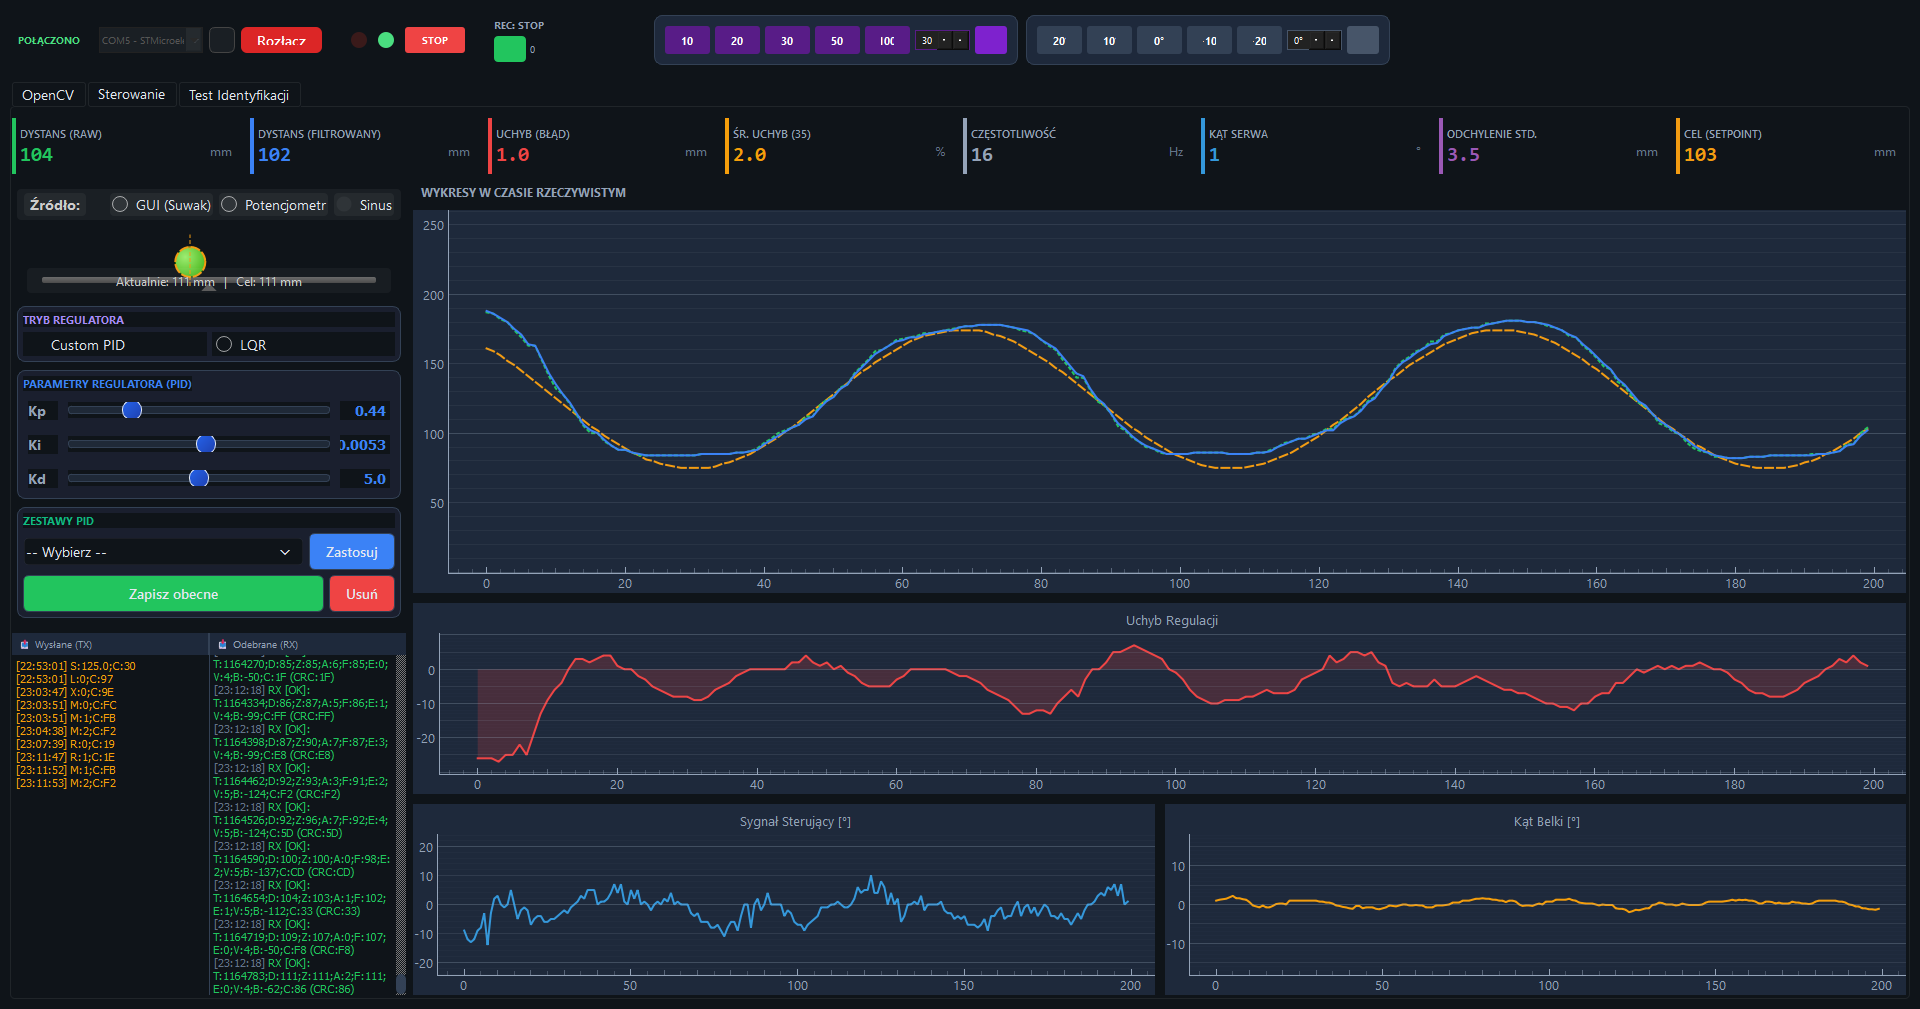
\includegraphics[width=0.9\linewidth]{2-budowa-stanowiska-i-oprogramowanie/2-img/desktop.png}
  \caption{Okno aplikacji desktopowej (PySide6)}
  \label{fig:desktop}
\end{figure}

% TODO: dodać zrzut ekranu zakładki wizyjnej aplikacji (opencv_panel)

% -----------------------------------------------------------------------
\section{Implementacja algorytmu sterowania}
% -----------------------------------------------------------------------

\subsection{Pętla sterowania i okres próbkowania}

Algorytm sterowania realizowany jest przez \texttt{ControlTask} z~ustalonym
okresem próbkowania 30\,ms????TODO wymuszonym przez funkcję \texttt{osDelay()}:

\begin{lstlisting}[style=cstyle, caption={Stały okres próbkowania w pętli sterowania (main.c)}]
#define PID_DT_MS 30

for (;;) {
    distance = readRangeContinuousMillimeters(&distanceStr);

    // obliczenia regulatora ...

    SetServoAngle(pid_output);
    osDelay(PID_DT_MS); // staly okres 30 ms
}
\end{lstlisting}

\subsection{Ograniczenie zakresu serwa}

Wyjście regulatora jest nasycane do bezpiecznego zakresu kąta serwa:

\begin{lstlisting}[style=cstyle, caption={Saturacja wyjścia i ograniczenia serwa (main.c)}]
#define SERVO_MIN_LIMIT  60.0f
#define SERVO_MAX_LIMIT 140.0f

if (pid_angle < SERVO_MIN_LIMIT)  pid_angle = SERVO_MIN_LIMIT;
if (pid_angle > SERVO_MAX_LIMIT)  pid_angle = SERVO_MAX_LIMIT;
SetServoAngle(pid_angle);
\end{lstlisting}

\subsection{Protokół telemetrii UART z sumą kontrolną CRC-8}

Dane pomiarowe przesyłane są przez UART~3 (115200\,baud) w~formacie
tekstowym z~sumą kontrolną CRC-8 (wielomian 0x07).
Format ramki:
\[
\texttt{D:\%d;Z:\%d;A:\%d;F:\%d;E:\%d;V:\%d;S:\%d;C:\%02X\textbackslash r\textbackslash n}
\]
gdzie kolejne pola oznaczają: surowy dystans, setpoint, kąt serwa,
dystans filtrowany, uchyb, średni uchyb, status czujnika i~CRC.

\begin{lstlisting}[style=cstyle, caption={Implementacja CRC-8 (crc8.c)}]
uint8_t CalculateCRC8(const char *data, int len) {
    uint8_t crc = 0x00;
    for (int i = 0; i < len; i++) {
        crc ^= data[i];
        for (uint8_t j = 0; j < 8; j++) {
            if (crc & 0x80)
                crc = (crc << 1) ^ 0x07;
            else
                crc <<= 1;
        }
    }
    return crc;
}
\end{lstlisting}

\subsection{Zadania FreeRTOS}

System operacyjny czasu rzeczywistego tworzy dwa wątki:

\begin{lstlisting}[style=cstyle, caption={Tworzenie zadań FreeRTOS (main.c)}]
osThreadDef(defaultTask, StartDefaultTask,
            osPriorityNormal, 0, 256);
defaultTaskHandle = osThreadCreate(osThread(defaultTask), NULL);

osThreadDef(ControlTask, StartControlTask,
            osPriorityHigh, 0, 1024);
ControlTaskHandle = osThreadCreate(osThread(ControlTask), NULL);

osKernelStart();
\end{lstlisting}

\section{System wizyjny}
\label{sec:wizja}

Stanowisko wyposażone jest w~podsystem wizji komputerowej realizujący bezdotykowy
pomiar pozycji kulki oraz kąta nachylenia belki.
Akwizycja i~przetwarzanie obrazu realizowane są po stronie aplikacji desktopowej
(Python\,/\,OpenCV), a~wyniki przesyłane są do mikrokontrolera przez interfejs UART. 

tutaj jakis screen z apki @piotrku 

% -----------------------------------------------------------------------
\subsection{Konfiguracja kamery i akwizycja obrazu}
% -----------------------------------------------------------------------

Akwizycja obrazu realizowana jest za pomocą funkcji \texttt{cv2.VideoCapture}
z~biblioteki OpenCV.
Kamera konfigurowana jest na stałą rozdzielczość 640$\times$480 pikseli
i~częstotliwość 30\,FPS z~minimalnym buforem klatek (\texttt{CAP\_PROP\_BUFFERSIZE = 1})
w~celu minimalizacji opóźnienia pomiarowego.
Aplikacja obsługuje automatyczne wykrywanie dostępnych kamer (tryb auto)
lub ręczny wybór indeksu urządzenia przez użytkownika.
Przetwarzanie kolejnych klatek wyzwalane jest przez timer Qt uruchamiany
z~jak największą częstotliwością.

% -----------------------------------------------------------------------
\subsection{Detekcja kulki metodą progowania w przestrzeni HSV}
% -----------------------------------------------------------------------

Kulka (piłeczka ping-pongowa) wykrywana jest na podstawie koloru
w~przestrzeni barw HSV (\emph{Hue, Saturation, Value}).
Przetwarzanie każdej klatki przebiega w~następujących krokach:

\begin{enumerate}
  \item \textbf{Rozmycie gaussowskie} — redukcja szumów; jądro $21\times21$\,px.
  \item \textbf{Konwersja BGR\,$\to$\,HSV} (\texttt{cv2.cvtColor}).
  \item \textbf{Progowanie zakresu barwy} (\texttt{cv2.inRange}):
    $H \in [8,\,64]$, $S \in [27,\,141]$, $V \in [121,\,255]$.
  \item \textbf{Operacje morfologiczne} — domknięcie (MORPH\_CLOSE) i~otwarcie
    (MORPH\_OPEN) na jądrze eliptycznym $5\times5$\,px; usuwają drobne
    artefakty i~wypełniają luki w~obrysie kulki. TUTAJ COS DOPSIAC @piotrku
  \item \textbf{Wykrywanie konturów} (\texttt{cv2.findContours}) — wybierany
    jest kontur o~największym polu; jeśli przekracza próg obszaru minimalnego
    (1480\,px\textsuperscript{2}), wyznaczane jest minimalne koło okalające
    (\texttt{cv2.minEnclosingCircle}).
\end{enumerate}

W~celu zmniejszenia czasu obliczeniowego stosowany jest dynamiczny obszar
zainteresowania (ROI): w~każdej klatce przeszukiwane jest okno $\pm100$\,px
wokół ostatnio wyznaczonej pozycji kulki, a~pełny obraz skanowany jest tylko
przy utracie śledzenia.
Podgląd maski HSV oraz obrazu wynikowego z~zaznaczoną kulką przedstawiony
jest na rys.~\ref{fig:wizja_hsv}.

\begin{figure}[H]
  \centering
  \fbox{\rule{0pt}{4cm}\rule{0.75\linewidth}{0pt}}
  \caption{Widok zakładki detekcji kulki: obraz oryginalny (lewy górny),
           maska HSV (prawy górny) oraz wynik z~zaznaczonym okręgiem (dolny)}
  \label{fig:wizja_hsv}
\end{figure}

@piotrku

% -----------------------------------------------------------------------
\subsection{Wyznaczanie pozycji belki na podstawie znaczników ArUco}
% -----------------------------------------------------------------------

Na ramie stanowiska przyklejone są cztery kwadratowe znaczniki ze słownika
\texttt{DICT\_4X4\_50}:
ID\,0 (prawy koniec belki), ID\,1 i~ID\,3 (punkty referencyjne ramy)
oraz ID\,2 (lewy koniec belki).
Detekcja znaczników realizowana jest przez moduł \texttt{cv2.aruco.ArucoDetector}
z~następującymi ustawieniami poprawiającymi wykrywanie małych i~zacienionych markerów:

\begin{itemize}
  \item preprocessing CLAHE (adaptacyjne wyrównanie histogramu lokalnego) na każdym
    wycinku ROI markera — lepsze radzenie sobie z~nierównomiernym oświetleniem;
  \item skalowanie podpikselowe ($\times3$) i~wyostrzanie jądrem $3\times3$
    przed detekcją; @piotrku co to jest skalowanie podpikselowe xd???
  \item precyzyjne dopasowanie narożników metodą AprilTag
    (\texttt{CORNER\_REFINE\_APRILTAG});
  \item rozluźnione progi geometryczne (dopuszczalna deformacja markera,
    minimalna długość krawędzi 0,1\,\% szerokości obrazu).
\end{itemize}

Każdy ze znaczników śledzony jest w~osobnym dynamicznym ROI o~marginesie 30\,px.
Mechanizm \emph{position holding} pozwala utrzymać ostatnio wyznaczoną pozycję
markera przez maksymalnie 15 klatek przy chwilowej utracie widoczności,
co zapobiega skokom w~pomiarze kąta.
Rozmieszczenie znaczników na stanowisku przedstawione jest na rys.~\ref{fig:wizja_aruco}.

\begin{figure}[H]
  \centering
  \fbox{\rule{0pt}{4cm}\rule{0.75\linewidth}{0pt}}
  \caption{Stanowisko z~nałożonymi wykrytymi znacznikami ArUco: ID\,2 (lewy koniec),
           ID\,0 (prawy koniec), ID\,1 i~ID\,3 (punkty referencyjne ramy)}
  \label{fig:wizja_aruco}
\end{figure}

@piotrku 

% -----------------------------------------------------------------------
\subsection{Kalibracja geometryczna i przeliczanie piksel $\to$ mm}
\label{subsec:kalibracja_wizja}
% -----------------------------------------------------------------------

Pozycja kulki wyznaczana jest jako rzut prostokątny jej środka na oś belki
(odcinek łączący środki znaczników ID\,2 i~ID\,0):

\begin{equation}
  t = \frac{(\mathbf{p} - \mathbf{A}) \cdot (\mathbf{B} - \mathbf{A})}
           {\|\mathbf{B} - \mathbf{A}\|^2},
  \quad t \in [0,\;1],
  \label{eq:rzut}
\end{equation}

gdzie $\mathbf{p}$ to współrzędne środka kulki w~pikselach,
$\mathbf{A}$ i~$\mathbf{B}$ to odpowiednio środki ID\,2 i~ID\,0.

Parametr $t$ przeliczany jest na milimetry za pomocą kalibracji dwupunktowej:
użytkownik umieszcza kulkę kolejno przy lewym i~prawym końcu belki,
rejestrując wartości $t_{\min} = 0{,}039$ i~$t_{\max} = 0{,}990$.
Wzór konwersji: @piotrku czy te wartosci powinny byc tutaj wpisane???

\begin{equation}
  x_{\mathrm{mm}} =
    \frac{t - t_{\min}}{t_{\max} - t_{\min}} \cdot L,
  \label{eq:kalibracja}
\end{equation}

gdzie $L = 250\,\mathrm{mm}$ jest długością aktywnej części belki.

Kąt nachylenia belki wyznaczany jest jako kąt odcinka ID\,2--ID\,0
względem poziomu obrazu (metoda domyślna) lub względem linii referencyjnej
ID\,1--ID\,3 (metoda alternatywna dostępna z~GUI).
Parametry kalibracji zapisywane są do pliku \texttt{opencv\_params.json}
i~wczytywane automatycznie przy kolejnym uruchomieniu aplikacji.

% -----------------------------------------------------------------------
\subsection{Protokół komunikacyjny PC $\to$ STM32}
% -----------------------------------------------------------------------

Wyniki pomiaru (pozycja kulki i~kąt belki) przesyłane są do mikrokontrolera
przez ten sam port szeregowy UART (115200\,baud), którym odbywa się telemetria
z~STM32.
Format ramki wizyjnej:

\begin{equation*}
  \texttt{V:\%d.\%d;B:\%d.\%d;C:\%02X\textbackslash n}
\end{equation*}

gdzie \texttt{V} to pozycja kulki w~mm, \texttt{B} to kąt belki w~stopniach,
a~\texttt{C} to suma kontrolna CRC-8 (wielomian 0x07) obejmująca pola
\texttt{V} i~\texttt{B}.
Ramki wysyłane są z~częstotliwością 30\,Hz przez dedykowany timer Qt.

Po stronie firmware funkcja \texttt{ParseVisionFrame()} (plik \texttt{main.c})
odróżnia ramkę wizyjną od standardowych komend sterujących po pierwszym znaku~\texttt{V},
waliduje CRC i~aktualizuje zmienne globalne \texttt{g\_vision\_ball\_pos}
i~\texttt{g\_vision\_beam\_angle}.
Jeśli przez ponad 200\,ms nie nadejdzie żadna poprawna ramka wizyjna,
regulator automatycznie przechodzi w~tryb fallback: jako pomiar pozycji
używana jest ostatnia poprawna wartość, a~kąt belki przyjmuje wartość $0 \deg$. @piotrku nie wiem czemu tutaj nie robi sie stopien

\begin{lstlisting}[style=cstyle, caption={Fragment funkcji ParseVisionFrame() (main.c) — parsowanie i walidacja CRC}]
void ParseVisionFrame(const char *frame) {
    // ...parsowanie pol V i B...
    if (crc_found && ball_pos >= 0.0f) {
        uint8_t crc_calc = CalculateCRC8(frame, data_len);
        if (crc_calc == crc_received) {
            g_vision_ball_pos   = ball_pos;
            g_vision_beam_angle = beam_angle;
            g_vision_data_valid = 1;
            g_vision_last_update = HAL_GetTick();
        }
    }
}
\end{lstlisting}

